\chapter{Experiments}\label{chapter:experiments}

% TODO: is it finetuning or training?

In this chapter we test several settings of the training method we introduced in
Chapter~\ref{chapter:training_method} and test each variant by evaluating the
trained models on downstream tasks. The goal of this chapter is to find the best
performing hyperparameters of our training method while trying to outperform
both teachers as well as the base student's checkpoint.

This chapter is laid out as follows. First we describe the training data and its
format in Section~\ref{section:val_training_data}. Second we define how we compare
models in Section~\ref{section:validation_tasks}. Third we describe the base
configuration of the student model along with the baselines, whose score we are
trying to exceed, in Section~\ref{section:student_model_config_baselines}. Then
we experiment with the structural loss in Section~\ref{section:structural_loss}.
Finally with the structural loss already given, we find the best performing
contextual loss and the weighting of the two losses in
Section~\ref{section:improving_both}.

\section{Training data}\label{section:val_training_data}

The training dataset for our validation experiments, which we label as
\Dataset{val\_500k}, is created in the same way as our final training dataset
\Dataset{train\_1500k} in Chapter~\ref{chapter:evaluation} except for the number
of containing documents. In short, we equally sample two sources that were used
to train our base student model: English Wikipedia and RealNews
articles~\citep{zellers2019defending} with documents longer than or 1200
Longformer tokens. We use our base student's training data, so that any
performance gains of the student model over its base checkpoint, can be
attributed to our training method, rather than to a higher quality training
dataset.

As can be seen in Table~\ref{table:val_data_stats}, \Dataset{val\_500k} is a
collection of large documents; the mean token count per document is over 1300
and around 65\% of the documents could not be processed by a traditional
Transformer such as RoBERTa~\citep{liu2019roberta} or SBERT. The distribution of
document length is far from uniform as we show in
Figure~\ref{fig:val_data_dist}.

\begin{table}
  \centering
  \begin{tabular}{lrr}
\toprule
Split & Train & Validation \\
\midrule
Documents & 500 000 & 10 000 \\
Tokens & 6.85e+08 & 1.37e+07 \\
Tokens per document & 1370.74$\pm$1723.38 & 1371.65$\pm$1717.24 \\
SBERT tokens over 384 & 70.56\% & 70.07\% \\
SBERT tokens over 512 & 66.37\% & 66.14\% \\
\bottomrule
\end{tabular}

  \caption{Statistics of \Dataset{val\_500k}. For each split we also show the
  percentage of documents with the number of SBERT tokens above given
  threshold.}

  \label{table:val_data_stats}

\end{table}

\begin{figure}

  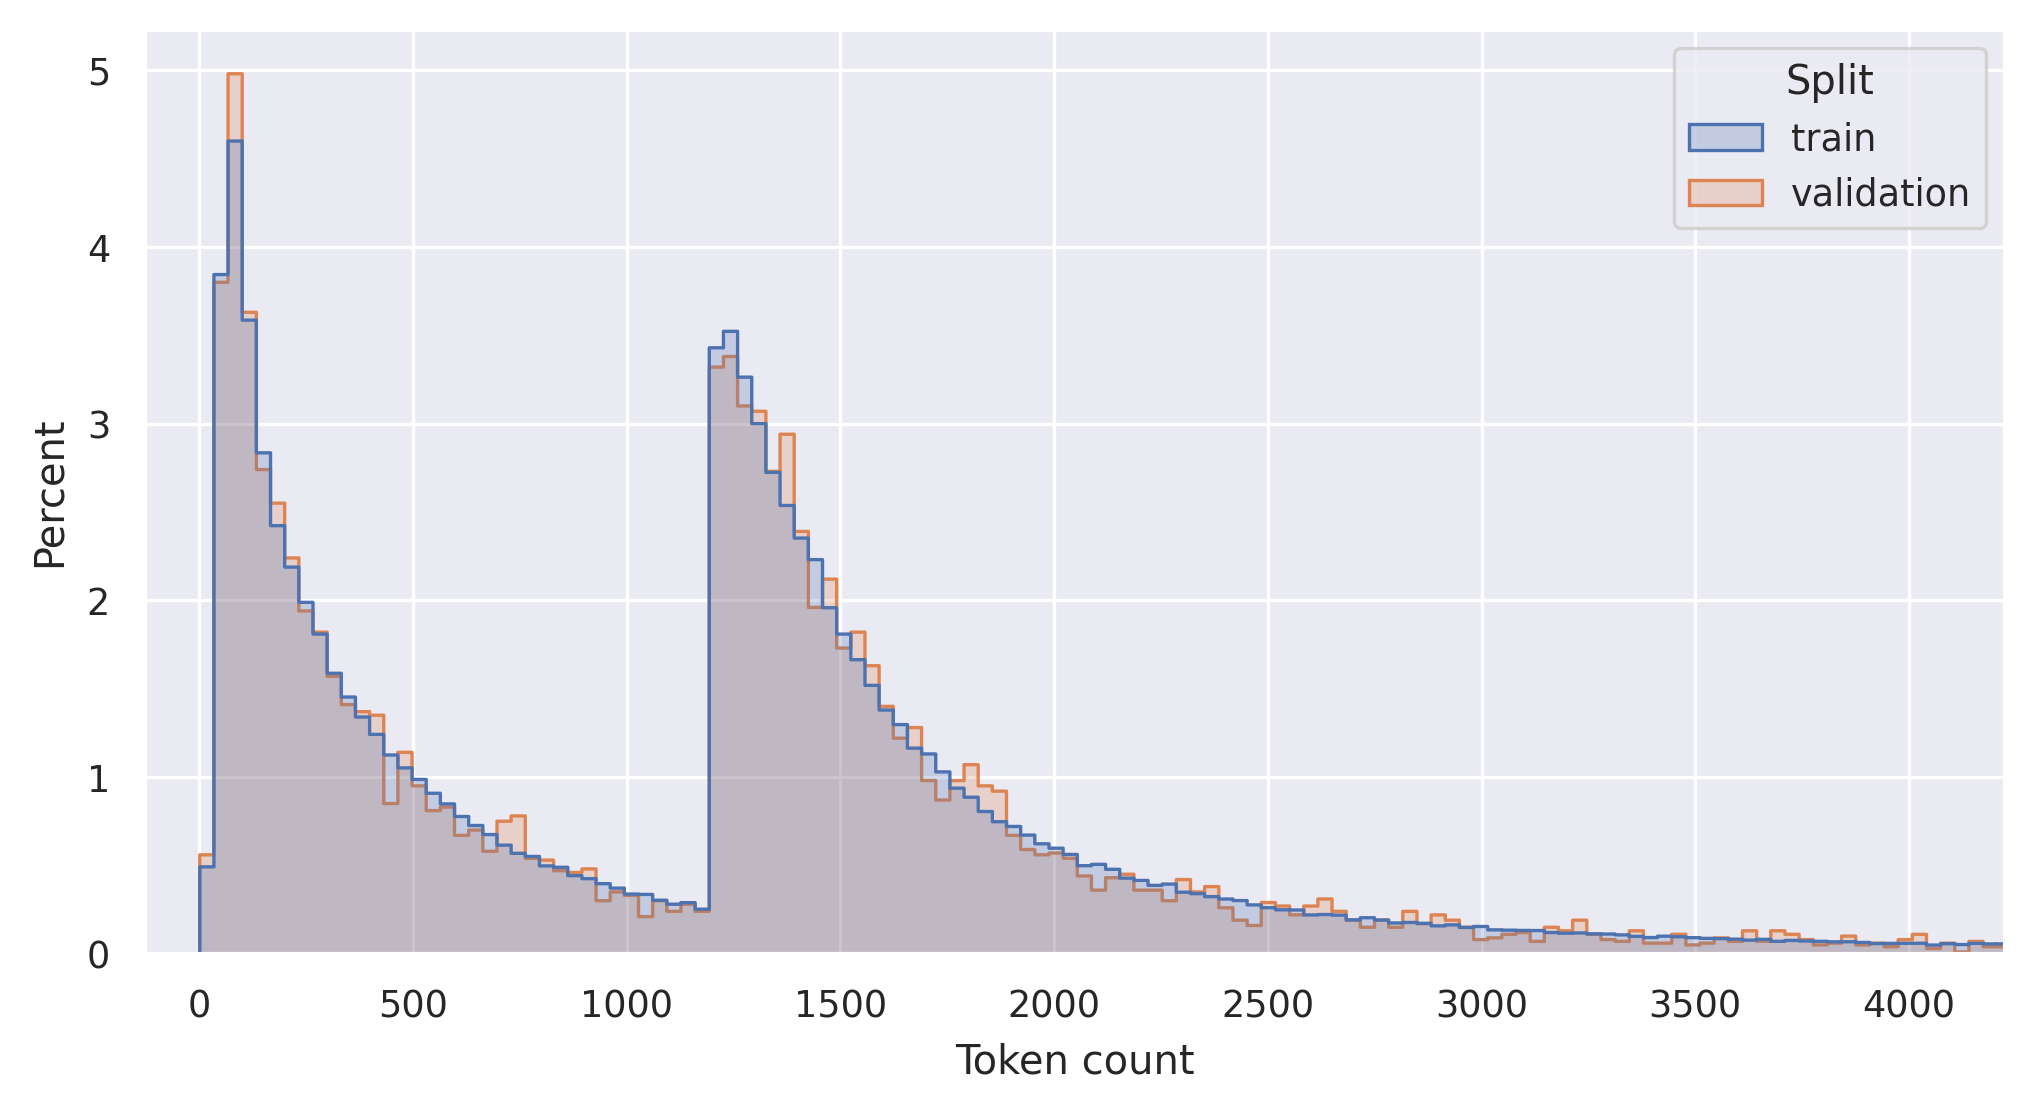
\includegraphics[width=\textwidth]{./img/val_data_dist.png}

  \caption{2-peak distribution of number of Longformer tokens per document in
    \Dataset{val\_500k}.}

  \label{fig:val_data_dist}

\end{figure}

\section{Validation tasks}\label{section:validation_tasks}

% I decided not to mention metrics here because:
%   - the metrics are tied to the losses used (COS, MSE, CCA, ...), that
%   haven't been explained yet
%   - even if they were there is nothing surprising that we track our loss
%   (essentially)
%   - the reader doesn't really need to know that we track them, once we need
%   to reference a metric (point to a graph or whatever), we just explain
%   what is what. The sole information that we track the metrics is useless.

We compare the training variants we compare the trained models' performances on
a set of downstream tasks. The set is composed of our evaluation tasks, which we
describe in Chapter~\ref{chapter:evaluation}, that either have large enough
training split suitable for cross-validation or validation split. We tabulate
the chosen tasks in Table~\ref{table:validation_tasks}. All tasks are
classifications and most are scored using a validation split, except for
\Task{IMDB} where we take the mean score of 5-fold cross-validation runs.

To make the validation process quicker we downsample the validation and train
splits to 10000 examples. We downsample the datasets according to their label
distribution, so that the truncated split has nearly identical label
distribution to the original one. We show the number of documents in each task
in Table~\ref{table:validation_tasks_statistics}. In the same table, we also
highlight the percentage of documents with above 384 SBERT tokens. These numbers
show how many documents must be truncated to fit into the context size of our
structural teacher $\Teacher_S$ and therefore also for how many documents we can
expect $\Teacher_S$ to receive full information and to give, perhaps, more
meaningful embeddings.

We use binary or micro-averaged accuracy as the scoring metric. Often we need to
compare performance across several tasks. However not all tasks are equally
difficult and so averaging accuracies would lead us to favoring models that
performed well on easy tasks, and undervaluing models that performed well on the
more difficult tasks. Therefore, we normalize the accuracy by the highest score
reached for the given task within the considered models and thereby making the
tasks equally difficult. We call this metric \emph{normalized accuracy}.

When validating a trained embedding model on a task we finetune a head that
transforms the embeddings into the output format required by the given task.
During validation we do not finetune the embedding model itself. Besides
speeding up the validation, this gives us also more genuine picture of the
performance of the embedding model. Since all our validation tasks are
classifications, the heads are just 2-layer neural network classifiers with a
cross-entropy loss. We give the complete list of classifier's hyperparameters
and training parameters in Table~\ref{table:head_train_params}.

TODO: ask if class distribution graph would add anything or not
\begin{table}
  \footnotesize
  \centering
\begin{tabular}{llrrr}
    \toprule
    \multicolumn{3}{r}{} & \multicolumn{2}{c}{Class percentage} \\
    \cline{4-5}
    Dataset & Evaluation & Classes & Train & Validation \\
    \midrule
    \Task{arxiv}~\citep{arxiv_papers} & validation split & 11 & 9.09$\pm$1.24\% & 9.09$\pm$1.01\% \\
    \Task{imdb}~\citep{maas2011learning} & cross-validation & 2 & 50.00$\pm$0.00\% & - \\
    \Task{oc}~\citep{zhou2020multilevel} & validation split & 2 & 50.00$\pm$0.06\% & 50.00$\pm$0.15\% \\
    \Task{aan}~\citep{zhou2020multilevel} & validation split & 2 & 50.00$\pm$1.50\% & 50.00$\pm$4.57\% \\
    \Task{s2orc}~\citep{zhou2020multilevel} & validation split & 2 & 50.00$\pm$0.09\% & 50.00$\pm$0.32\% \\
    \Task{pan}~\citep{zhou2020multilevel} & validation split & 2 & 50.00$\pm$0.00\% & 50.00$\pm$0.00\% \\
    \bottomrule
\end{tabular}

  \caption{Validation tasks used in this chapter. Each task is evaluated either
    using a validation split or cross-validated on training split using 5 folds.
    The class distributions of all tasks are well balanced except for \Task{aan}
    as can be seen from the mean and standard deviation of class percentages for
    given task and split.}

  \label{table:validation_tasks}

\end{table}

\begin{table}
  \footnotesize
  \centering
\begin{tabular}{llrrr}
\toprule
 Dataset & Split & Documents & Over 384 tokens & Over 512 tokens \\
\midrule
\multirow[c]{2}{*}{\Task{arxiv}} & Train & \dag10 000 & 100.00\% & 100.00\% \\
 & Test & 2 500 & 100.00\% & 100.00\% \\
\cline{1-5}
\Task{imdb} & Train & \dag10 000 & 24.34\% & 14.63\% \\
\cline{1-5}
\multirow[c]{2}{*}{\Task{oc}} & Train & \dag10 000 & 12.22\% & 1.00\% \\
 & Test & \dag10 000 & 12.38\% & 1.05\% \\
\cline{1-5}
\multirow[c]{2}{*}{\Task{aan}} & Train & \dag10 000 & 0.51\% & 0.03\% \\
 & Test & \dag10 000 & 0.34\% & 0.07\% \\
\cline{1-5}
\multirow[c]{2}{*}{\Task{s2orc}} & Train & \dag10 000 & 33.23\% & 18.40\% \\
 & Test & \dag10 000 & 32.94\% & 18.67\% \\
\cline{1-5}
\multirow[c]{2}{*}{\Task{pan}} & Train & \dag10 000 & 72.72\% & 63.37\% \\
 & Test & 2 908 & 59.99\% & 45.34\% \\
\cline{1-5}
\bottomrule
\end{tabular}

    \caption{The statistics of validation tasks used in this chapter. We truncated
    splits marked with {\dag} to speed up validation of models. We truncate a
    split by downsampling it according to its label distribution. For each split
    we give a percentage of documents with number of SBERT tokens above given
    threshold.}

    \label{table:validation_tasks_statistics}

\end{table}

\begin{table}
  \centering
  \begin{tabular}{l c}
    \toprule
    Parameter & Value \\
    \midrule
    Hidden features & 50 \\
    Hidden dropout rate & 0.5 \\
    Hidden activation & ReLU \\
    Epochs & 10 \\
    Batch size & 32 \\
    Weight decay & 0.1 \\
    Label smoothing & 0.1 \\
    Learning rate & 1e-4 \\
    Learning rate decay & Cosine \\
    Maximum gradient norm & 1.0 \\
    Optimizer & AdamW \\
    Mixed-precision training & Yes \\
    \bottomrule
  \end{tabular}

  \caption{Hyperparameters and training parameters of classification heads used
    during validation.}

  \label{table:head_train_params}

\end{table}

\section{Student's model configuration and baselines}\label{section:student_model_config_baselines}

As we explained in Section~\ref{section:student_model}, we chose
Longformer~\citep{beltagy2020longformer} as our student model. We use
Longformer's smaller base version with about 126M parameters implemented by
HuggingFace \texttt{datasets}
library\footnote{\url{https://huggingface.co/allenai/longformer-base-4096}}.

To obtain the input's embedding we average the final hidden states. We do not
use global attention and restricting ourselves to only sliding window attention,
with the window sizes $\omega$ set to the default 512 tokens. During training of
the student model we aim for fast convergence with small memory footprint. We
therefore use high learning rate, no gradient accumulation steps,
mixed-precision training and gradient checkpointing. The complete list of
training parameters is displayed in Table~\ref{table:student_train_params}.


\begin{table}
  \centering
  \begin{tabular}{l c}
    \toprule
    Parameter & Value \\
    \midrule
    Batch size & 6 \\
    Weight decay & 0.1 \\
    Learning rate & 1e-4 \\
    Learning rate decay & Cosine \\
    Maximum gradient norm & 1.0 \\
    Optimizer & AdamW \\
    Gradient accumulation steps & 1 \\
    Warmup steps & 10\% of training steps \\
    Gradient checkpointing & Yes \\
    Mixed-precision training & Yes \\
    \bottomrule
  \end{tabular}

  \caption{Parameters for training student models during validation experiments.
    We use these values unless specified otherwise.}

  \label{table:student_train_params}

\end{table}

\subsection{Baselines}

As we already mentioned in the beginning of this chapter, the goal of the
following experiments is to find out weather we can surpass both teachers as
well as the base checkpoint of our student model using our teacher-student
training approach. To that end we compare our student model throughout this
chapter to three models: SBERT~\citep{reimers2019sentence},
Longformer~\citep{beltagy2020longformer} and PV~\citep{le2014distributed}. For
SBERT we use the same version and checkpoint as for our structural teacher. For
Longformer we use the same configuration we use for our student model. For
Paragraph Vector we use the same model and checkpoint as for our contextual
teacher, which we train in Section~\ref{section:gen_contextual_embeds}.

\section{Structural loss}\label{section:structural_loss}

% what it does
% why is it more important than contextual loss
% we should 'squeeze' out of it all that it has got -> absolute similarity
% options -- name each, give results for each
%   - mse
%   - cos
%
% We won't mention max-marginal type of losses because:
%   - according to metrics they are not the best and we would have hard time
%   arguing why we chose them instead of the vanilla versions
%   - only cosine works, mse needs more work
%   - and even cosine could be improved by having more negatives than just
%   in-batch
%   - all this needs time we don't have
%   - so if it will be included, it will be as an ablation study
%   - the other option is to not limit ourselves to just metrics, and just
%   evaluate them on validation splits

To limit the number of hyperparameter combinations, we first experiment with
structural loss only and after finding the best performing $\Loss_S$ we start
using both losses at the same time, finetuning both $\Loss_C$ and $\lambda$.
This approach is based on our initial experiments, where the structural teacher
proved to be more important to the performance of the student model than the
contextual teacher. We therefore finetune the contextual loss to the already
given structural loss instead of the other way around.


The structural loss $\Loss_S$ compares the embeddings of the student $\Student$
to those of the structural teacher $\Teacher_S$. As we mentioned in
Section~\ref{section:abstract_loss} we want $\Loss_S$ to minimize the distance
between the two embeddings as much as possible.

We considered two basic losses: Mean Squared Error (or MSE) and cosine
distance.


While MSE forces the two
embeddings to be identical, cosine distance only forces the embeddings to have
the same direction.

The structural loss $\Loss_S$ is one of the two losses our teacher-student
training will use. For inputs that fit into the maximum context length of the
structural teacher, the structural loss should minimize the dissimilarity
between the structural teacher's and the student's embeddings as much as
possible. This follows our assumption that for inputs that the structural model
can process whole, the structural model produces an embedding with the deepest
understanding of the input that is available to us. It is thus important that
the similarity $\mathcal{L}_D$ should take into account is the absolute
similarity rather than some approximate measure of it.

(TODO: What else to say about this? What dissimilarity we use will be in
Experiments chapter as well as deciding "when an input is applicable".)


\section{Improving both qualities at the same time}\label{section:improving_both}

After finding the best performing variant of $\Loss_S$, our goal is to find the
best performing $\Loss_C$. Instead of experimenting with just the contextual
loss, we train models with both losses used. So in essence, we look for a
variant of $\Loss_C$ that will complement the already chosen $\Loss_S$ the best,
rather than looking for the overall best performing $\Loss_C$.

First we train the contextual teacher $\Teacher_C$ in the next section. In the
following sections we experiment with $\Loss_C$ and with the weighting of the
structural and contextual losses.


\subsection{Generating contextual embeddings}\label{section:gen_contextual_embeds}


As we have explained in Section~\ref{section:paragraph_vector}, we have chosen
Paragraph Vector~\citep{le2014distributed} as our contextual teacher. Since
there is no concept of pre-training, as in the case of transformers, we train PV
from scratch. We use the implementation provided by Gensim
library\footnote{\label{fn:link_to_gensim}\url{https://radimrehurek.com/gensim}}.


\subsubsection{Grid searching best performing hyperparameters}

There is a great number of hyperparameters governing the training of Paragraph
Vector. We focus only on four hyperparameters, while following the
recommendations of related literature or leaving the parameter to its default
value, sensibly set by the Gensim library authors. Both the adopted and the
grid-searched hyperparameters are displayed in Table~\ref{table:pv_hyperparams},
where the mentioned hyperparameters have the following meaning:

\begin{itemize}

  \item \texttt{dm} --  PV architecture; true for Distributed Memory (DM),
    false for Distributed Bag of Words (DBOW)

  \item \texttt{vector\_size} -- dimensionality of the generated embedding

  \item \texttt{min\_count} -- words with document frequency below this limit
    will be ignored

  \item \texttt{text\_pre\_process} -- applied word processing done before the
    model's training; for stemming we used PorterStemmer implemented by
    \texttt{nltk}
    library\footnote{\url{https://www.nltk.org/api/nltk.stem.porter.html}}

  \item \texttt{negative} -- number of noise words used for negative sampling
    during training

  \item \texttt{window} -- the maximum distance between known and predicated
    word

  \item \texttt{sample} -- percentile threshold configuring which words will be
    downsampled; 0 for no downsampling


  \item \texttt{dbow\_words} -- whether to train word embeddings using
    Word2Vec~\citep{mikolov2013efficient} Skip-gram architecture simultaneously
    with DBOW document embeddings

  \item \texttt{epochs} -- number of iterations over the corpus

\end{itemize}


We train both DM and DBOW as recommended by the authors of Paragraph
Vector~\citep{le2014distributed}. \texttt{vector\_size}, \texttt{min\_count} and
\\ \texttt{text\_pre\_process} all control the regularization of the model.
Settings such as higher dimensional embedding, small min count and no text
pre-processing, regularize the model the least. They give the model the most
information on its inputs, while also providing it with large embedding through
which the model can express in more detail. On the other hand, using lower
dimensional embedding, large minimal count and heavy text pre-processing, forces
the model to be more general and less precise. The model has less detailed
information on its input and must squeeze all of it to a small vector. We did
not see any value in trying higher dimensions of embeddings than 1024 as in
later experiments we need to distill the contextual embedding to a
768-dimensional embedding of our student model. Intuitively, the larger the
contextual embedding is going to be, the smaller the percentage of information
the student model is going to be able to digest. Also there is no value in
considering \texttt{min\_count} to be lower than 2, since we would only add
words that are unique to a single document. Embeddings of such words would be
poorly trained and would not add meaningful information to the document's
embedding. Last hyperparameter that deserves mention is \texttt{dbow\_words}.
DBOW on its own does not train word embeddings, which are randomly generated.
Setting \texttt{dbow\_words} to true causes DBOW to also train word embeddings
using Word2Vec Skip-gram model in each epoch. \cite{lau2016empirical} showed
that random word embeddings hurt the model significantly, and so in our opinion
the overall longer training, with \texttt{dbow\_words} set to true, is worth the
performance gain.

\begin{table}
  \footnotesize
  \centering
  \begin{tabular}{lrc}
    \toprule
    Hyperparameter & Value(s) & Recommended by \\
    \midrule
    \texttt{dm} & true, false & - \\
    \texttt{vector\_size} & 100, 768, 1024 & - \\
    \texttt{min\_count} & 2, 10\% of train corpus & - \\
    \texttt{text\_pre\_process} & stem, lowercase, none & - \\
    \texttt{window} & 5 & default \\
    \texttt{negative} & 5 & default, \cite{lau2016empirical} \\
    \texttt{sample} & 0 & default \\
    \texttt{dbow\_words} & true & \cite{lau2016empirical} \\
    \texttt{epochs} & 10 & default, \cite{dai2015document} \\
    \bottomrule
  \end{tabular}

  \caption{Used hyperparameters for training Paragraph Vector. We grid-searched
  four hyperparameters: PV architecture, vector size, min. word count and
  pre-processing of words. The rest of the hyperparameters we adopted either the
  default values set by the authors of the Gensim
  library\textsuperscript{\ref{fn:link_to_gensim}} or recommended by the
  mentioned literature.}

  \label{table:pv_hyperparams}

\end{table}

We train all variants on the entire \Dataset{val\_500k} corpus. We report the
normalized classification for each variant in Figure~\ref{fig:pv_val_scores}.
Large embedding dimensions and low minimum count were favored. There is no clear
preference among the types of pre-processing. DBOWs vary more in performance,
occupying the best and the worst positions, whereas DMs are a bit more
consistent.

\begin{figure}
    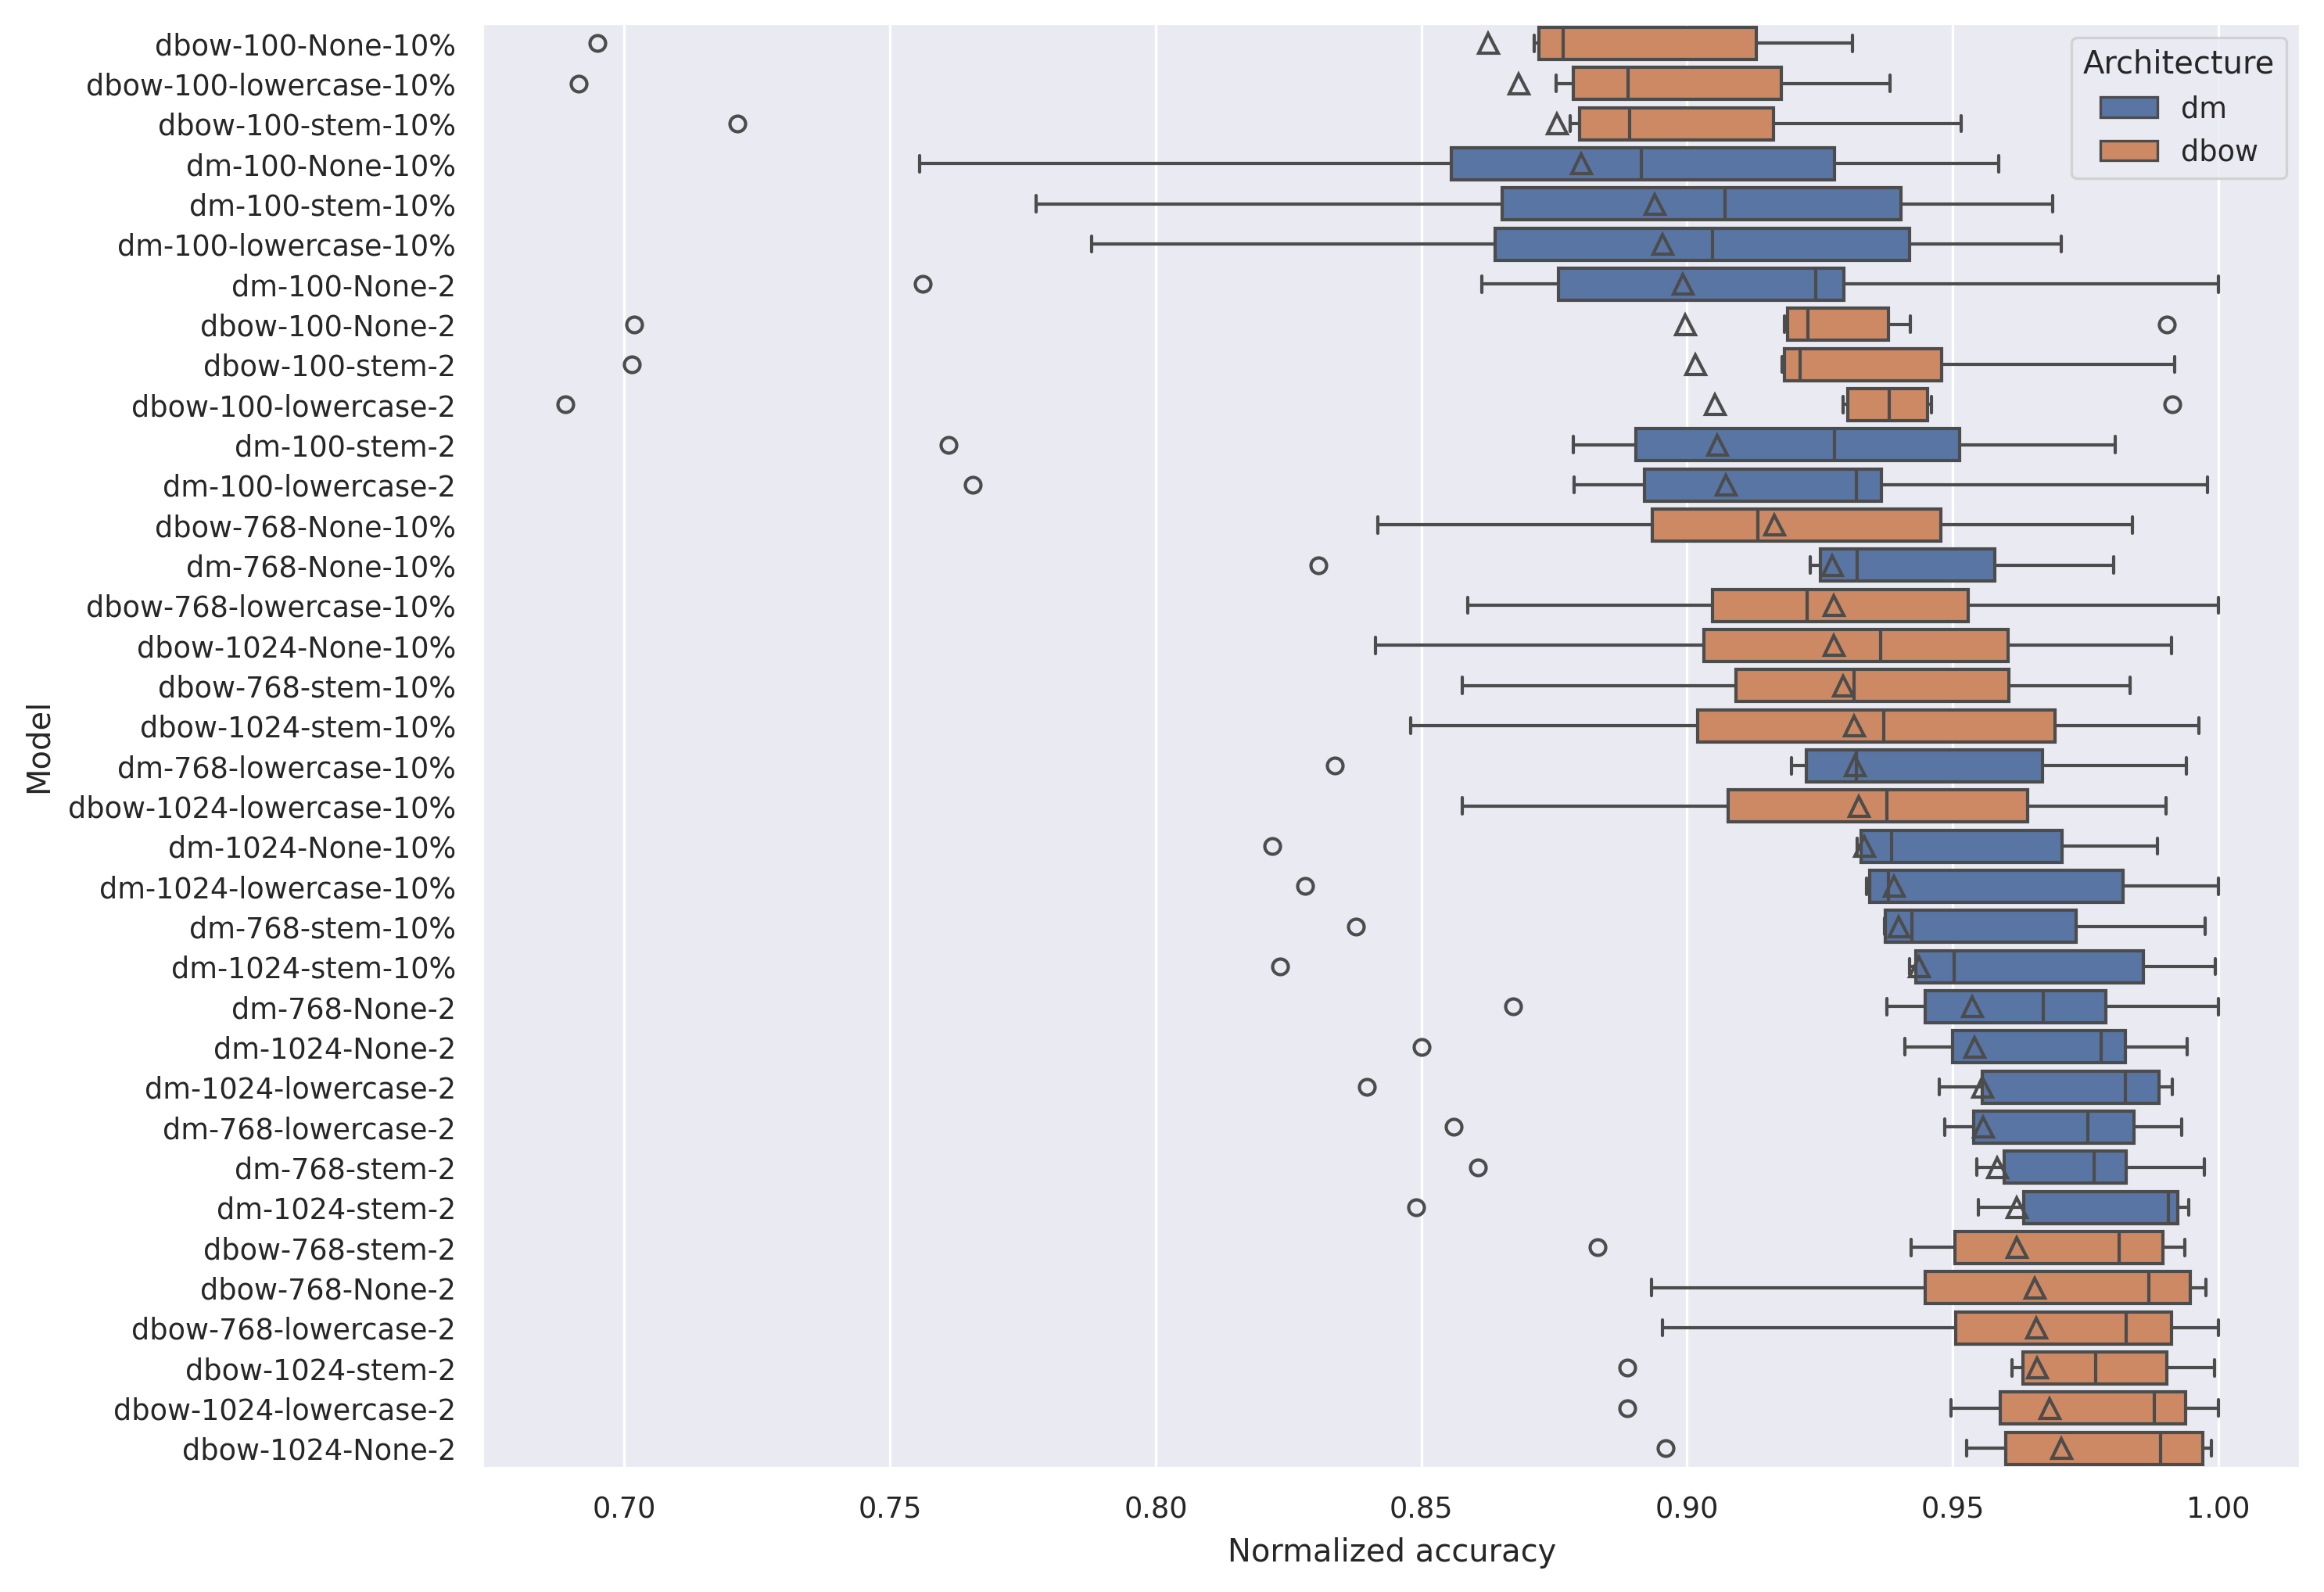
\includegraphics[width=\textwidth]{./img/pv_val_scores.png}

    \caption{Boxplot of normalized accuracies of all PV models on validation
    tasks. Model is identified by architecture, embedding dimension, text
    pre-processing and minimum count, in this order, delimited by a hyphen. The
    models are sorted according to the mean normalized accuracy marked with a
    triangle.}

    \label{fig:pv_val_scores}
\end{figure}

\textbf{Will we actually do the concatenation? There is an opportunity to make
up some time, which I don't have enough of. Also I thing the argument ``we need
to cramp this huge (2048d) contextual embedding down into 768d student
embedding'' is pretty sound.}

\subsubsection{Training the contextual teacher}

We take the best performing hyperparameter values from the previous section and
train the model on a large corpora. As we later train our student model with the
contextual teacher's outputs, each piece of data we train our contextual model
with, is effectively also part of the student's training data. Therefore we
construct the PV training dataset similarly as \Dataset{val\_500k}: we evenly
sample English Wikipedia articles and RealNews~\citep{zellers2019defending}
articles with more than 1200 Longformer tokens. We do so for the same reasons
that were mentioned in Section~\ref{section:val_training_data}.

Since PV is a small model and is able to process data very quickly during
training, we can afford to use all of the RealNews articles that are long enough
and an equal amount of Wikipedia articles. This results in a corpus that has
8.3M documents. We train the model for 10 epochs, but restrict the maximum
  vocabulary size to $1.2{\times}10^7$ words to limit the memory footprint to
  roughly 140~GB.

\subsection{Structural loss selection}

The contextual loss $\mathcal{L}_B$ minimizes the disagreements between the
embeddings of the contextual teacher model  and that of the student model.
There are two major differences between the contextual loss and the structural
loss. First the contextual loss is always applicable. It might not be the loss
that reflects our ultimate goal the most for the given input. Nevertheless we
still assume that for \emph{every} input the contextual teacher model offers
some information which the structural teacher model does not have. Second the
contextual loss is not as exact as the structural loss. Instead of forcing the
teacher model to adhere to two possibly very distinct ways how to encode
information into a dense vector representation, we give the model a little bit
of freedom. We do so by letting the model decide how exactly it should encode
the information contained in the contextual teacher's embedding. We give the
model more leeway on the breadth side rather than the structural side, because
we expect that the precision of the embedding is more important than capturing
every piece of the input.

With the above taken into an account we chose to use a variant of
\emph{Canonical Correlation Analysis}~\cite{hotelling1992relations} (or
\emph{CCA}) as a base for our breath loss $\mathcal{L}_B$. A variant of CCA fits
our needs very nicely as it computes a correlation of outputs after some
projection. While the projection gives the model the freedom to restructure its
embeddings, the correlation ensures that the two embeddings agree with each
other. Before going further let us briefly describe CCA and its variants we
considered.

\subsubsection{Canonical Correlation Analysis}

Canonical Correlation Analysis (CCA) computes linear projections of two vectors
such that their projections are maximally correlated. For formal definition
reference Definition~\ref{def:cca}.

\begin{defn}[Canonical Correlation Analysis]\label{def:cca}

  For two matrices $X_1 \in \mathbb{R}^{n_1 \times m_1}$ and $X_2 \in
  \mathbb{R}^{n_2 \times m_1}$, Canonical Correlation Analysis finds $p \in
  \mathbb{R}^m_1$ and $q \in \mathbb{R}^m_2$ that maximize

  \begin{equation}
    \begin{split}
      & corr(X_1p, X_2q) = \frac{p^TX_1^TX_2q}{||Xp|| ||Yq||} \\
      \text{s.t.}\quad &||X_1p|| = ||X_2q|| = 1 \\
    \end{split}
  \end{equation}


\end{defn}

Definition~\ref{def:cca} suggests that CCA gives only a single number as the
measure of correlation of two matrices. When the dimensions of the input vectors
are large enough, however, often there exists at least one combination of
features that results in correlation of 1. As this would make CCA relatively
useless in the context of high-dimensional spaces we assume multiple
correlations for several mutually orthogonal projections. We name such Canonical
Correlation analysis as CCA for more dimensions and define it formally in
Definition~\ref{def:cca_more_dim}

\begin{defn}[Canonical Correlation Analysis for more dimensions]\label{def:cca_more_dim}

  For two matrices $X_1 \in \mathbb{R}^{n_1 \times m_1}$ and $X_2 \in
  \mathbb{R}^{n_2 \times m_1}$, Canonical Correlation Analysis for $k$
  dimensions finds $P \in \mathbb{R}^{m_1 \times k}$ and $Q \in \mathbb{R}^{m_2
  \times k}$ that maximize

  \begin{equation}
    \begin{split}
      &\sum_{i = 1}^k corr(X_1P_{*i}, X_2Q_{*i}) \\
      \text{s.t.}\quad &P^TX_1^TX_1P = I_k = Q^TX_2^TX_2Q \\
    \end{split}
  \end{equation}


\end{defn}

If we consider the conditions in Definition~\ref{def:cca_more_dim}, the
resulting value can be easily reformulated:

\begin{equation}
    \sum_{i = 1}^k corr(X_1P_{*i}, X_2Q_{*i}) =
    trace(P^TX_1^TX_2Q) =
    trace(P^T\Sigma_{X_1X_2}Q)
\end{equation}

Where $\Sigma_{X_1X_2}$ is the covariance matrix of $X_1$ and $X_2$.

TODO: analytical solution to pure CCA

As we noted above we would like to use CCA as a base for our contextual loss
$\mathcal{L}_B$ in order to establish correspondence between the contextual
teacher's embedding and the student's. The problem using CCA as it was defined
in Definition~\ref{def:cca_more_dim} as a loss is that it is defined in the
context of the whole dataset rather than just a minibatch. It is therefore
unclear how should be CCA computed using just a pair of minibatches.

Someone (TODO: citation) found that using large enough batch size is sufficient
for the training to converge.

\subsubsection{Deep CCA}

Deep CCA (or DCCA) is an extension of CCA that computes projections using
neural networks. As such it is more powerful than plain CCA as it allows for
non-linear projections. To compute DCCA the network has to be trained on the
pairs of vectors with CCA as its loss.

TODO: graphic of architecture

If CCA is weaker condition than just correlation, DCCA is even weaker since
there is no limit to how the projections should look like.

\subsubsection{Soft CCA}

Soft CCA reformulates CCA and thus allows its straightforward use in the
context of minibatches. With constraints from Definition~\ref{def:cca_more_dim}
taken into account, CCA can be formulated using Forbenious matrix norm:

\begin{align}
  P^\ast, Q^\ast &= \underset{P, Q}{\argmin} ||X_1P - X_2Q||^2_F \\
  &= \underset{P, Q}{\argmin} trace\Big((X_1P - X_2Q)^T(X_1P - X_2Q)\Big) \\
  &= \underset{P, Q}{\argmin} {-2} trace(P^TX_1^TX_2Q) \\
  &= \underset{P, Q}{\argmax} trace(P^TX_1^TX_2Q) \\
  &= \underset{P, Q}{\argmax} \sum_{i = 1}^k corr(X_1P_{*i}, X_2Q_{*i})
\end{align}

So, in essence minimizing CCA is the same as minimizing the difference between
projections, whose features are decorrelated. This is the formulation Soft CCA
builds on. Soft CCA decomposes CCA into to parts:

\begin{itemize}
  \item minimization of the difference between projections

    \begin{equation}
      ||X_1P - X_2Q||^2_F
    \end{equation}

  \item decorrelation of each projection $P$

    \begin{equation}
      \sum_{i \ne j} (P^TX^T_{mini}X_{mini}P)_{ij} = \sum_{i \ne j} \Sigma_{X_{mini}P},
    \end{equation}

    where $X_{mini}$ is batch-normalized minibatch.

\end{itemize}

To bring correlation matrix of the current minibatch $\Sigma_{X_{mini}P}$
closer to the true covariance, the decorrelation part is in fact computed from
a covariance matrix that is incrementally learned.

In this way Soft CCA incrementally decreases CCA through incrementally learned
approximation of the projections' covariances.

\subsubsection{Loss selection}

\begin{itemize}
    \item mention which of the CCA variants we chose
    \item reiterate the formulation in the context of teacher-student training
\end{itemize}
% finetune loss + projection together but separately
% for each loss

\subsubsection{Mean Squared Error}
\subsubsection{Vanilla CCA}
\subsubsection{SoftCCA}
\subsection{Balancing structural and contextual}
% Length balancing goes here


\section{Ablation studies}

\begin{itemize}
  \item here we can ablate some parts of our method (e.g. training with just
    the contextual teacher)
\end{itemize}
